\documentclass[a4paper,12pt,twoside]{article}
\usepackage[left=1in,right=1in,top=1in,bottom=1in]{geometry}

\usepackage{xeCJK}
\setCJKmainfont{Songti TC}
\setCJKfamilyfont{kai}{Songti TC}
\newcommand{\kai}{\CJKfamily{kai}} % 用 \kai{使用楷書}

\usepackage{lmodern}
\usepackage{titling}
\usepackage{titlesec}
\usepackage{graphicx}
\usepackage{float}
\usepackage{amsmath, amsthm, amssymb, amsfonts, mathrsfs}
\usepackage{upgreek} % 直立的希臘字母

\usepackage[shortlabels]{enumitem}
\usepackage{setspace}
\renewcommand{\baselinestretch}{1.5}
\usepackage[colorlinks]{hyperref}
\usepackage{fancyvrb}
\usepackage{fancyhdr}
\usepackage{multicol}
\usepackage{caption}
\usepackage{listings}
\usepackage{bm}
\usepackage{bbm} % for \mathbbm{1} (indicator function)
\usepackage{centernot}
\usepackage{mdframed}
\usepackage{tikz}
\usetikzlibrary{patterns, arrows.meta, positioning}
\usepackage[nameinlink, capitalise]{cleveref}
\usepackage{diagbox}
\usepackage{booktabs}
\usepackage{multirow,array}
\usepackage{tabularx}
\usepackage{mathtools}
\usepackage{indentfirst} % 首段 indent
\setlength{\parindent}{2em}
\usepackage{cancel} % 數學式子畫線槓掉
\newcommand\mcancel[2][red]{\setbox0=\hbox{$#2$}%
\rlap{\raisebox{.45\ht0}{\textcolor{#1}{\rule{\wd0}{1pt}}}}#2}
\usepackage{datetime2}

\AtBeginDocument{%
 \setlength{\abovedisplayskip}{6pt}
 \setlength{\belowdisplayskip}{6pt}
 \setlength{\abovedisplayshortskip}{4pt}
 \setlength{\belowdisplayshortskip}{4pt}
}

\definecolor{codegreen}{rgb}{0,0.6,0}
\definecolor{codegray}{rgb}{0.5,0.5,0.5}
\definecolor{codepurple}{rgb}{0.58,0,0.82}
\definecolor{backcolour}{rgb}{0.95,0.95,0.92}

\lstdefinestyle{mystyle}{
 backgroundcolor=\color{backcolour},
 commentstyle=\color{codegreen},
 keywordstyle=\color{magenta},
 numberstyle=\tiny\color{codegray},
 stringstyle=\color{codepurple},
 basicstyle=\ttfamily\footnotesize,
 breakatwhitespace=false,
 breaklines=true,
 captionpos=b,
 keepspaces=true,
 numbers=left,
 numbersep=5pt,
 showspaces=false,
 showstringspaces=false,
 showtabs=false,
 tabsize=2
}
\lstset{style=mystyle}

\hypersetup{citecolor=blue, linkcolor=blue, urlcolor=blue}

\DeclareMathOperator{\supp}{supp}
\DeclareMathOperator{\skewness}{Skewness}
\DeclareMathOperator{\DU}{D-U}
\DeclareMathOperator{\CU}{C-U}
\DeclareMathOperator{\Geo}{Geo}
\DeclareMathOperator{\Pois}{Pois}
\DeclareMathOperator{\Gam}{Gam}
\DeclareMathOperator{\LN}{LogN}
\DeclareMathOperator{\cov}{Cov}
\DeclareMathOperator*{\argmax}{arg\,max}
\DeclareMathOperator*{\argmin}{arg\,min}
\DeclareMathOperator{\re}{Re}
\DeclareMathOperator{\im}{Im}

\newcommand{\N}{\mathbb{N}}
\newcommand{\Z}{\mathbb{Z}}
\newcommand{\Q}{\mathbb{Q}}
\newcommand{\R}{\mathbb{R}}
\newcommand{\C}{\mathbb{C}}
\newcommand{\G}{\mathcal{G}}
\newcommand{\mP}{\mathbb{P}}
\newcommand{\F}{\mathcal{F}}
\newcommand{\B}{\mathcal{B}}
\newcommand{\1}{\mathbbm{1}}
\newcommand{\Poi}{\text{Poi}}
\newcommand{\Var}{\text{Var}}
\newcommand{\as}{\text{a.s.}}
\newcommand{\vect}[1]{\boldsymbol{\mathbf{#1}}}
\newcommand{\paren}[1]{\left({#1}\right)}
\newcommand{\brk}[1]{\left[{#1}\right]}
\newcommand{\curl}[1]{\left\{{#1}\right\}}
\renewcommand{\lambda}{\lambdaup}

\theoremstyle{definition} % 定理環境 style 改用正體
\newtheorem{theorem}{定理}
\newtheorem{definition}{定義}
\newtheorem*{definition*}{定義}
\newtheorem{example}{例子}
\newtheorem{exercise}{練習}
\newtheorem{corollary}{推論}
\newtheorem{property}{性質}
\newtheorem{prop}{命題}
\newtheorem{lemma}{引理}
\newtheorem{problem}{問題}
\newtheorem*{remark}{註}

\renewcommand{\figurename}{圖}
\renewcommand{\tablename}{表}

\DeclareMathOperator{\var}{Var}
\DeclareMathOperator{\corr}{corr}
\DeclareMathOperator{\rank}{rank}
\DeclareMathOperator{\MSE}{MSE}
\DeclareMathOperator{\SSE}{SSE}
\DeclareMathOperator{\SST}{SST}
\DeclareMathOperator{\SSR}{SSR}
\DeclareMathOperator{\sgn}{sign}
\DeclareMathOperator{\alt}{Alt}
\DeclareMathOperator{\adj}{adj}
\DeclareMathOperator{\curlOp}{curl}
\DeclareMathOperator{\spn}{span}
\DeclareMathOperator{\sse}{SSE}
\DeclareMathOperator{\tr}{tr}

\newcommand{\ep}{\varepsilon}
\newcommand{\p}{\partial}
\newcommand{\abs}[1]{\left|#1\right|}
\newcommand\norm[1]{\left\lVert#1\right\rVert}
\newcommand{\innerprod}[1]{\langle#1\rangle}
\newcommand{\ds}{\displaystyle}
\newcommand{\blank}{\rule[-1mm]{1.5cm}{0.1mm}}
\newcommand{\dint}{\displaystyle\int}
\renewcommand{\bar}{\overline}

\newtheoremstyle{remark}{}{}{}{}{\bfseries\sffamily}{.}{.5em}{#1}
\theoremstyle{remark}

\newtheorem*{remark*}{\textit{Remark}}
\newtheorem*{solution*}{解}

\AtEndEnvironment{solution*}{\hfill$\square$}
\newtheorem*{hint*}{Hint}


\newcommand{\redtext}[1]{{\color{red} #1}}
\newcommand{\bluetext}[1]{{\color{blue} #1}}

\fancypagestyle{firstpage}{
  \fancyhf{}
  \fancyhead[R]{\small《高中數學實驗教材》第 2 冊}
  \fancyhead[L]{\small 第 2 章\quad 次序與極限觀念}
  \fancyfoot[C]{\thepage}
}

\pagestyle{fancy}
\setlength{\headheight}{14pt}
\renewcommand{\headrulewidth}{0.5pt}
\renewcommand{\footrulewidth}{0pt}
\fancyhead{}
\fancyhead[LE]{\small 《高中數學實驗教材》第二冊}
\fancyhead[RO]{\small 第二章\quad 次序與極限觀念}
\fancyfoot[C]{\thepage}

\title{\LARGE\textbf{《高中數學實驗教材》第二冊}\\[0.5em] \Large\textbf{第二章\quad 次序與極限觀念}}
\author{\textbf{高中數學實驗教材編輯小組}\quad 編著}
\date{民國六十二年（1973）初版}

\begin{document}

\maketitle
\thispagestyle{firstpage}

% ==========================================
% 掃描檔勘誤、文字校訂與疑難處說明（依規則整理於目錄之前）
% ==========================================
\section*{【說明】掃描檔勘誤、疑難處與文義校訂表}
\addcontentsline{toc}{section}{【說明】掃描檔勘誤、疑難處與文義校訂表}
\label{sec:errata_notes}

本章依據 1973 年版《高中數學實驗教材 第二冊》（高一下）第二章「次序與極限觀念」掃描原件轉錄為 \LaTeX{} 格式。為忠實反映教材原始內容並兼顧排版品質與嚴謹性，依作業規範將掃描檔中出現之印刷訛誤、符號缺漏、字模損毀、歷史印記雜訊及文義疑難處詳細考證彙整於下表。讀者可點擊表格中之章節連結直接跳至正文對應位置：

\begin{table}[H]
\centering
\small
\renewcommand{\arraystretch}{1.35}
\begin{tabularx}{\textwidth}{|p{3.2cm}|p{3.6cm}|X|}
\hline
\textbf{章節位置} & \textbf{掃描檔原始現象 / 誤植} & \textbf{考證說明與校訂處理} \\ \hline

\hyperref[note:b2-ch2-p28-ex3-pr]{§ 1-2 頁 28 例 3} & 
「$b = \frac{pr}{sq}$ 且 $sq>0, ps>0, pr>0$」及「$n(ps)>pr$」 & 
通分時分子 $pr$ 實為 $qr$（因 $b=\frac{r}{s}=\frac{qr}{sq}$，通分後比較 $nps$ 與 $qr$），原書排印誤植為 $pr$。正文忠實照錄原書文字，特予考證備註。 \\ \hline

\hyperref[note:b2-ch2-p29-ex5-subscript]{§ 1-2 頁 29 例 5(ii)} & 
「現在寫做 $n+k=2_s$」 & 
式中 $2_s$ 之 $s$ 為下標，實為指數次方 $2^s$（2 的 $s$ 次方）之排版鉛字下標訛誤。正文忠實照錄原書文字 $2_s$，並在此說明。 \\ \hline

\hyperref[note:b2-ch2-p30-ex2-1-q2i]{§ 1-2 頁 30 習題 2-1 第 2(i) 題} & 
「$a>b \text{ 和 } c<0 \implies ac>bd$」 & 
前提中未定義變數 $d$（或係 $ac<bc$ 之排印訛誤，或脫漏 $b>0, c<d<0$ 等條件）。正文忠實保留原刊印文字，特予備註說明。 \\ \hline

\hyperref[note:b2-ch2-p37-ex3-typo]{§ 3 頁 37 例 3} & 
「$f(x)>0$ 的解是 $-1x<1$，及 $x>3$」 & 
式中「$-1x<1$」脫漏小於號「$<$」，實為 $-1<x<1$。正文照錄原書印刷字樣，並於此校釋。 \\ \hline

\hyperref[note:b2-ch2-p40-ex3-vi]{§ 4-1 頁 40 例 3(vi)} & 
「$0, 0, n, 0, 0, -n+1, 0, 0, -(n+1), \dots$ 為一數列」 & 
依每 6 項循環結構，第 $6n$ 項為 $-n$，第 $6n+3$ 項為 $n+1$，式中「$-n+1$」排印脫漏符號，實為「$-n, 0, 0, n+1$」。正文忠實保留原印文字並予考證。 \\ \hline

\hyperref[note:b2-ch2-p44-ex6-series-term]{§ 5-1 頁 44 例 6} & 
「級數 $1, r, r^2, r^3, r^4, \dots, r^n, \dots$ 的收斂與發散」 & 
此處列出者實為等比數列各項，行文稱「級數」，且後續條件稱「當 $r<1$ 時」，若 $r\le -1$ 則發散或震盪，係省略負數討論或隱含 $|r|<1$ 之意。正文忠實照錄原書文字。 \\ \hline

\hyperref[note:b2-ch2-p50-eq1-b1]{§ 6-1 頁 50 式 (1)} & 
「$= \frac{b_1}{1-r} + \frac{-r^n}{1-r} \dots\dots(1)$」 & 
第二項分子常數首項 $b_1$ 脫漏（應為 $\frac{-b_1 r^n}{1-r}$）。正文忠實照錄原印文字，並在此說明。 \\ \hline

\hyperref[note:b2-ch2-p51-lim-rn]{§ 6-1 頁 51 式 (2) 前} & 
「因此由（5-1）〔例 6〕$\frac{-r^n}{1-r} \to 0$」 & 
前文對應處實為 §5-1【例 6】。原書此處交叉引註形式保留不變。 \\ \hline

\hyperref[note:b2-ch2-p56-partial-sum-r]{§ 6-3 頁 56 部分和式} & 
「$= a_k + d(1+r+r^2+\dots+\frac{1}{r^{m-1}})$」 & 
式中括號末項誤植為分式 $\frac{1}{r^{m-1}}$，實為 $r^{m-1}$（因公比 $r=\frac{1}{10^l}$）。正文保留原書文字並予備註。 \\ \hline

\hyperref[note:b2-ch2-p56-q-typo]{§ 6-3 頁 56 分數化小數段} & 
「設 $\frac{m}{n}$ 為一任意給定的不可約分數……若 $q$ 上含有 2 或 5 的質因子」 & 
前設分數為 $\frac{m}{n}$，文內「若 $q$ 上含有」之 $q$ 顯為分母 $n$ 之誤植（後文亦稱「反之，若 $n$ 含有……」）。正文忠實照錄原書文字，特予考證備註。 \\ \hline

\end{tabularx}
\end{table}

\clearpage
\tableofcontents
\newpage

% =========================================================================
% 《高中數學實驗教材》第二冊（高一下） 
% 第二章 次序與極限觀念
% =========================================================================

\section{次序與極限觀念}\label{sec:b2_ch2}

「數系」的概念由於對於各種「量」的問題作有系統的討論而產生. 例如：吃了一根香蕉再吃一根香蕉，共吃了兩根香蕉，是一個日常生活的經驗，將它抽象化之後，我們便得到 $1+1=2$. 所以由「量與量之間的相加」抽象出來「數與數之間的加法運算」. 在第一冊第三章中，我們更談到如何以「加法運算」為基礎，逐步衍生出「減」、「乘」、「除」等運算. 日常生活的量與量之間，除了可以相加之外，還常有很自然的「大小」關係. 將這些關係抽象化，即得「數與數之間的次序關係」（亦即 $>$ 或 $<$ 關係）. 運算與次序關係是數系的兩種基本結構.

以數系在運算上所具有的基本性質為出發點，在上一冊以及這一冊的第一章中，我們討論過整數的因子分解、多項式的運算與因子分解以及一次、二次方程式的理論及應用. 本章將以數系在「次序關係」上的基本性質為出發點，逐步討論不等式與極限觀念. 同學們將會看出極限觀念也就是次序關係在觀念上的一種推廣.

\subsection{次序與不等式的基本性質}\label{sec:b2_2-1}

\subsubsection*{1-1 次序與正負}

在日常生活中，我們說 $A$ 量大於 $B$ 量的意義是：「從 $A$ 量減去 $B$ 量後還有剩餘.」所以在數系中我們定義「$a$ 大於 $b$」的意義為「$a-b$ 是一正數」. 也就是
\begin{definition*}
$a>b \iff a-b \text{ 是一正數}.$
\[
a<b \iff a-b \text{ 是一負數}.
\]
所以 $a>b$ 與 $b<a$ 是同一回事.
\end{definition*}

\paragraph{注意：} 由上述定義，我們有下面的特例
\begin{align*}
a>0 &\iff a \text{ 為一正數}, \\
a<0 &\iff a \text{ 為一負數}.
\end{align*}
這種正負數的表示法，前面已經用過.

在整數系、有理數系及實數系中，顯然都具有下列性質. 即
\begin{enumerate}[(i)]
    \item 正數加正數仍為正數.
    \item 正數乘正數仍為正數.
    \item 正數乘負數則為負數. \quad （符號定則）
    \item 負數乘負數則為正數.
    \item 任何一數或為正，或為零，或為負；且上述三種可能性互斥.
\end{enumerate}

\subsubsection*{1-2 不等式的基本性質}

基於上述五點關於正、負數的性質，我們說明不等式的基本性質如下：
\begin{enumerate}[(1)]
    \item $a>b \text{ 和 } b>c \implies a>c$.
    
    \noindent\textbf{【證明】} $a>b \text{ 和 } b>c \implies a-b>0 \text{ 和 } b-c>0$
    \[
    \overset{\text{(i)}}{\implies} a-c = (a-b)+(b-c) > 0 \implies a>c.
    \]

    \item 對任何兩數 $a, b$，由 (v) 可知下列關係有一種且僅有一種成立：
    \[
    a>b,\quad a=b,\quad \text{或 } a<b.
    \]

    \item $a>b \iff a+c > b+c$. \quad （註\footnote{性質 (3) 表示加法的對消法則對不等式也成立，因此移項法則也成立.}）
    
    \noindent\textbf{【證明】} 
    \begin{align*}
    a>b &\iff a-b=(a+c)-(b+c)>0 \\
    &\iff a+c>b+c.
    \end{align*}

    \item $a>b \text{ 和 } c>d \implies a+c>b+d$.
    
    \noindent\textbf{【證明】} 
    \begin{align*}
    a>b \text{ 和 } c>d &\implies a+c>b+c \text{ 和 } b+c>b+d \\
    &\overset{\text{(1)}}{\implies} a+c>b+d.
    \end{align*}

    \item $a>b \text{ 和 } c>0 \implies ac>bc$.
    
    \noindent\textbf{【證明】} 
    \begin{align*}
    a>b \text{ 和 } c>0 &\implies a-b>0, \text{ 和 } c>0. \\
    &\overset{\text{(ii)}}{\implies} ac-bc = (a-b)\cdot c > 0. \\
    &\implies ac>bc.
    \end{align*}

    \item $a>b \text{ 和 } c<0 \implies ac<bc$.

    \item $a>b>0,\ c>d>0 \implies ac>bd$.
\end{enumerate}

\begin{example}\label{ex:b2_2-1-1}
所有的正整數可以按大小次序排為 $1<2<3<\dots < k < k+1 < \dots$.
\end{example}

\begin{example}\label{ex:b2_2-1-2}
因為 $9>-13$，用上面的性質 (5) 得到 $9\times (-8) > (-13)\times(-8)$ 也就是 $-72>104$，錯誤在那裏？
\end{example}

\begin{example}\label{ex:b2_2-1-3}
對任意的正有理數 $a, b$，我們可以找到一個正整數 $n$，滿足 $na>b$.
\end{example}

\noindent\textbf{【證明】} 先假定 $a, b$ 都是正整數，我們利用正整數的除法，得到
\[
b=ka+r \qquad 0\le r < a
\]
如果讓 $n=k+1$，我們有
\[
(k+1)a-b = (k+1)a-ka-r = a-r > 0
\]
如果現在 $a=\frac{p}{q},\ b=\frac{r}{s}$，且 $q>0,\ s>0,\ p>0,\ r>0$.

因為 $a=\frac{ps}{sq}$ 和 $b=\frac{pr}{sq}$ 且 $sq>0, ps>0, pr>0$\phantomsection\label{note:b2-ch2-p28-ex3-pr}，如果找到 $n$，使得 $n(ps)>pr$. 那麼
\[
\frac{nps}{sq} > \frac{pr}{sq},\quad \text{也就是 } na>b.
\]

\paragraph{注意：} 這個例題叫做阿基米德性質，當我們學了實數的稠密性後，可以很容易的證明在正實數上也有阿基米德性質.

我們也可以考慮代數式之間的不等關係，譬如以下的例子：

\begin{example}\label{ex:b2_2-1-4}
若 $a, b$ 是正數，試證 $\frac{a+b}{2} \ge \sqrt{ab}$，且等式成立的充分必要條件是 $a=b$.
\end{example}

\noindent\textbf{【證明】} 因為 $(a-b)^2 \ge 0$，所以 $a^2-2ab+b^2 \ge 0$，將上式兩邊同加 $4ab$，我們有
\[
a^2+2ab+b^2 \ge 4ab
\]
\[
\frac{(a+b)^2}{4} \ge ab
\]
所以
\[
\frac{a+b}{2} \ge \sqrt{ab}
\]
如
\begin{align*}
\frac{a+b}{2} = \sqrt{ab} &\iff \frac{(a+b)^2}{4} = ab \\
&\iff (a-b)^2 = 0 \\
&\iff a-b = 0 \\
&\iff a = b.
\end{align*}

\begin{example}\label{ex:b2_2-1-5}
對於任意正數 $a_1, a_2, \dots, a_n$，我們有
\[
\frac{a_1+a_2+\dots+a_n}{n} \ge \sqrt[n]{a_1 a_2 \dots a_n}
\]
\end{example}

\noindent\textbf{【證明】} 
\begin{enumerate}[(i)]
    \item 由〔例 4〕我們知道 $n=2$ 時成立，$n=4$ 時
    \[
    \frac{\frac{a_1+a_2}{2}+\frac{a_3+a_4}{2}}{2} \ge \sqrt{\left(\frac{a_1+a_2}{2}\right)\left(\frac{a_3+a_4}{2}\right)}
    \]
    \[
    \left(\frac{a_1+a_2+a_3+a_4}{4}\right)^2 \ge \frac{a_1+a_2}{2}\cdot\frac{a_3+a_4}{2} \ge \sqrt{a_1 a_2}\sqrt{a_3 a_4}
    \]
    所以
    \[
    \frac{a_1+a_2+a_3+a_4}{4} \ge \sqrt[4]{a_1 a_2 a_3 a_4}
    \]
    利用歸納法，我們可以把上述情形延伸到所有的次方. 同學試自行討論.

    \item 假定 $n$ 不是 2 的次方，那麼我們可以將 $n$ 加一個正整數 $k$，使得 $n+k$ 是 2 的次方，現在寫做 $n+k=2_s$\phantomsection\label{note:b2-ch2-p29-ex5-subscript}
    
    我們令 $\alpha = \frac{a_1+a_2+\dots+a_n}{n}$，則 $\alpha$ 是正數，所以對 $2^s$ 個正數 $a_1, a_2, \dots, a_n, \underbrace{\alpha, \dots, \alpha}_{k\text{ 個}}$ 適用 (i) 的結果而得出
    \[
    \frac{a_1+a_2+\dots+a_n+k\alpha}{n+k} \ge \sqrt[n+k]{a_1 a_2 \dots a_n \alpha^k}
    \]
    也就是
    \[
    \frac{n\alpha+k\alpha}{n+k} \ge \sqrt[n+k]{a_1 a_2 \dots a_n \alpha^k}
    \]
    兩邊取 $n+k$ 次方，我們就有
    \[
    \alpha^{n+k} \ge a_1 a_2 \dots a_n \alpha^k
    \]
    消去 $\alpha^k$，得到 $\alpha^n \ge a_1 \dots a_n$
    也就是
    \[
    \left(\frac{a_1+a_2+\dots+a_n}{n}\right)^n \ge a_1 a_2 \dots a_n
    \]
    \[
    \therefore \frac{a_1+a_2+\dots+a_n}{n} \ge \sqrt[n]{a_1 a_2 \dots a_n}
    \]
\end{enumerate}

\paragraph{注意：} 「次序關係」（亦即 $>$, $<$ 關係）是數系的基本結構之一，所以不等式的演算和等式的演算在數學中具有同樣的重要性，是不容忽視的. 但是不等式在演算上和等式的演算有些不同的地方，同學們宜特別注意，多加小心，以免犯錯.
\begin{itemize}
    \item[（甲）] 性質 (5)，(6) 說明——當不等式的兩端同乘一正數時，不等式的方向不變，但是不等式的兩端同乘一個負數時，不等式的方向逆轉.
    \item[（乙）] 性質 (4) 說明——兩個同方向的不等式，可以兩端分別相加而得一原方向的不等式. 但是將兩個方向相反的不等式兩端分別相加時，任何情形（即 $>$, $=$, $<$）都可能產生.（請同學舉例說明）
    \item[（丙）] 性質 (7) 說明——若有方向相同的兩個不等式，而且每一不等式的兩端皆是正數，則將此兩不等式兩端分別相乘，仍得一原方向之不等式，但若不等式兩端的正負未能確定時，上述的結果一般不能成立.（請同學自己舉例討論）
\end{itemize}

\subsubsection*{習題 2-1}

\begin{enumerate}
    \item 將下列各數依大小次序排列：
    \[
    10^6,\quad 3^{12},\quad 2^{20}.
    \]

    \item 證明
    \begin{enumerate}[(i)]
        \item $a>b \text{ 和 } c<0 \implies ac>bd$.\phantomsection\label{note:b2-ch2-p30-ex2-1-q2i}
        \item $a>b>0,\ c>d>0 \implies ac>bd$.
    \end{enumerate}

    \item 定義 ``$a\ge b \iff a>b \text{ 或 } a=b$'' 而且 ``$a\le b \iff b>a,\ b=a$''. 請檢查一下，$\ge$ 與 $\le$ 是否滿足性質 (1) 到 (7).

    \item 若 $a, b, c$ 都是正數，試證明
    \[
    a^2+b^2+c^2 \ge ab+bc+ca,
    \]
    且等式成立的充分必要條件是 $a=b=c$.

    \item 設 $a, b, c$ 為不等的正數，證明
    \[
    a^3+b^3 > a^2 b+ab^2.
    \]

    \item 如果 $a, b, c$ 是不等的正數，試證明
    \[
    (a+b)(b+c)(c+a) > 8abc.
    \]

    \item 證明 $(a+b)(a^3+b^3) \ge (a^2+b^2)^2$，其中 $a, b$ 是正數.

    \item 證明 $\frac{a}{b}+\frac{b}{a} \ge 2$，其中 $a, b$ 是正數.

    \item 如果 $x, x', y, y'$ 都是實數，證明
    \[
    |xx'+yy'| \le \sqrt{(x^2+y^2)(x'^2+y'^2)}.
    \]

    \item 如果 $n$ 是正整數，$a, b$ 是正有理數，證明
    \[
    \frac{a^n+b^n}{2} \ge \left(\frac{a+b}{2}\right)^n.
    \]

    \item 設 $a>1$，而 $x, y$ 為正數，那麼
    \[
    a^{\frac{x+y}{2}} \text{ 和 } \frac{1}{2}(a^x+a^y) \text{ 那個大？}
    \]

    \item 上文〔例 5〕中等式成立的充分必要條件是
    \[
    a_1=a_2=\dots=a_n,
    \]
    請同學自行討論.
\end{enumerate}

\subsection{直線的坐標化}\label{sec:b2_2-2}

在上一節中，我們討論數系中數與數之間的大小關係. 其實這類的次序關係，並不僅限於數系中才有，在很多別的場合中，也是很常見的. 譬如一條水平直線上的點與點之間就具有左右關係.

\subsubsection*{2-1 數系次序關係與直線次序關係的比較}

直線上的次序關係如「$A$ 點在 $B$ 點之右」或「$C$ 點在 $B$ 點之左」寫起來很繁. 我們將仿照數系的性質，引入下列符號：

用「$A>B$」表示「$A$ 點在 $B$ 點之右」，

用「$C<B$」表示「$C$ 點在 $B$ 點之左」，

用「$A=B$」表示「$A$ 點與 $B$ 點相同」.

採用上述簡便符號，則下列事實可以改寫如下：
\begin{enumerate}[(i)]
    \item ``$A \text{ 在 } B \text{ 之右和 } B \text{ 在 } C \text{ 之右} \implies A \text{ 在 } C \text{ 之右}''$ 可改寫為
    \[
    ``A>B \text{ 和 } B>C \implies A>C''.
    \]
    \item 對於直線上任意兩點 $A, B$，下列關係有一種且僅有一種成立. 即「$A$ 在 $B$ 之右」，「$A, B$ 相同」或「$A$ 在 $B$ 之左」. 改寫後即成
    \[
    A>B,\quad A=B,\quad \text{或 } A<B.
    \]
\end{enumerate}

直線次序關係所具有的上述兩個性質顯然和上一節所講的數系次序關係的性質 (1)、(2) 完全一樣（註\footnote{至於數系次序關係的其他五個性質（即 (3) — (7)），它們涉及加乘運算. 但是直線上的點與點之間沒有自然的運算，因而也就談不上運動有沒有相當於 (3) — (7) 這些性質了.}）. 更進一步，在本節中我們要利用直線坐標化，來說明數系與水平線依次序關係的觀點來看，具有相同的構造.

\subsubsection*{2-2 直線坐標化}

直線坐標化的步驟如下：

\noindent (一) 在直線上取定一點作為基準點，叫做坐標系的原點. 習慣上以大寫字母「$O$」代表它. 它的坐標規定為 0.

\begin{figure}[H]
\centering
\begin{tikzpicture}[x=1.4cm, y=1cm]
    % Axis line
    \draw[thick, <->] (-4.2, 0) -- (4.2, 0);

    % Unit length indicator
    \draw[|-|, thick] (0, 0.9) -- (1, 0.9) node[midway, above=2pt] {\small 單位長};

    % Coordinates and tick marks
    \foreach \x/\lbl in {
        -3.8/b,
        -3/-3,
        -2.5/-a,
        -2/-2,
        -1.414/-\sqrt{2},
        -1/-1,
        0/0,
        1/1,
        1.414/\sqrt{2},
        2/2,
        2.5/a,
        3/3
    } {
        \draw[thick] (\x, 0.12) -- (\x, -0.12);
        \node[above=2pt] at (\x, 0.12) {$\lbl$};
    }

    % Bottom labels
    \node[below=4pt] at (-3.8, -0.15) {$B$};
    \node[below=4pt] at (0, -0.15) {$O$};
    \node[below=4pt] at (2.5, -0.15) {$A$};

    % Direction labels below
    \node at (-2, -0.9) {左};
    \node at (0, -0.9) {(原點)};
    \node at (2, -0.9) {右};
\end{tikzpicture}
\end{figure}

\noindent (二) 我們取定一個線段作為單位長，並且：
\begin{itemize}
    \item[] 原點之右，距原點 1 單位的點的坐標規定為 1，
    \item[] 原點之左，距原點 1 單位的點的坐標規定為 $-1$，
    \item[] 原點之右，距原點 2 單位的點的坐標規定為 2，
    \item[] 原點之左，距原點 2 單位的點的坐標規定為 $-2$，
\end{itemize}
以此類推.

位於原點右方 $\sqrt{2}$ 單位處的點的坐標規定為 $\sqrt{2}$，

位於原點左方 $\sqrt{2}$ 單位處的點的坐標規定為 $-\sqrt{2}$，$\dots$ 等等.

換句話說：
\begin{itemize}
    \item[] $A$ 點的坐標為 $a$，$a>0$ 乃是表示 $A$ 點位於原點右方 $a$ 單位處.
    \item[] $B$ 點的坐標為 $b$，$b<0$ 乃是表示 $B$ 點位於原點左方 $|b|$ 單位處.
\end{itemize}

對於直線的坐標，有下列幾點事實：
\begin{enumerate}[(i)]
    \item 對應於直線上一條給定的點，由它和原點間的相對位置（亦即距離與左、右）決定一個實數，叫做該點的坐標.
    \item 反之，對應於一個給定的實數，也決定直線上一點，其坐標為該給定的實數.
    \item 上述直線上的點和實數間的一一對應叫做直線上的\textbf{一個坐標系}. 它利用實數系去有系統的表示直線上的點.
    \item 設 $A$ 點的坐標是 $a$，$B$ 點的坐標是 $b$，則
    \[
    \overline{AB} = A, B \text{ 之間的距離} = |a-b|;
    \]
    \[
    A \text{ 在 } B \text{ 之右} \iff A>B \iff a>b;
    \]
    \[
    A \text{ 在 } B \text{ 之左} \iff A<B \iff a<b.
    \]
    \item 當我們選取不同的點作為基準點（就是坐標系原點）或不同長度為單位長時，就得到直線上不同的坐標系. 所以在一條直線上存在有許多坐標系. 我們可以隨討論的問題而選定較為方便的坐標系.
\end{enumerate}

\subsubsection*{習題 2-2}

\begin{enumerate}
    \item 設數集 $A=\{x \mid -1 \le x \le +1\}$, $B=\{x \mid x>0\}$，分別在直線上描出對應於 $A, B$, $A\cup B$, $A\cap B$ 的點集.

    \item 如果 $AB$ 兩點的坐標各為 $a, b$，求
    \begin{enumerate}[(a)]
        \item 中點 $C$ 的坐標，
        \item 求 $k-1$ 個 $k$ 等分點的坐標.
    \end{enumerate}

    \item （槓桿原理）：如果在一箇桿子上兩點 $A, B$ 上分別掛上重量等於 $p, q$ 公斤的物品，假設 $A, B$ 的坐標分別是 $a, b$，請問支點（也就是重心）的坐標應該是多少才能平衡？（假定桿子的重量可以忽略不計）

    \item 在一條直線上，取 $O$ 為原點，$OE$ 為單位長（$E$ 點的坐標是 1）. 設 $O'$ 的坐標是 3.5，$E'$ 的坐標是 4.5，如果我們取 $O'$ 為新的原點，$\overline{O'E'}$ 為新的單位長，得到一個新的坐標系，問 $O$ 點、$E$ 點在新坐標系中的坐標是什麼？又如果 $P$ 點在舊坐標系中坐標是 $p$，問在新坐標系中坐標是什麼？

    \item 在一直線上有二個坐標系 (I)、(II)，如果二個坐標系的原點 $O$ 與 $O'$ 是同一個點，但是坐標系 (I) 中的單位長是坐標系 (II) 中單位長的 $\sqrt{2}$ 倍，問一點 $P$ 在坐標系 (I)、(II) 中的坐標 $p_1, p_2$ 有怎樣的關係？

    \item 在一直線上給予兩個坐標系 (I) 和 (II)，設任意一點 $P$ 在坐標系 (I) 中的坐標是 $x_1$，在坐標系 (II) 中的坐標是 $x_2$. 證明有兩個實數 $a, b$ ($a\ne 0$) 存在，使得 $x_2 = ax_1+b$. （這個式子叫做坐標變換公式）

    \item 在直線上給予兩個坐標系 (I)、(II)，設兩點 $P, Q$ 在 (I) 中的坐標是 $2, 8$，在 (II) 中的坐標是 $3, 5$，求這兩種坐標間變換的公式.
\end{enumerate}

\subsection{不等方程式}\label{sec:b2_2-3}

在很多工程上或日常的問題中，常常出現不等式. 譬如有一座吊橋，鐵索上所承受的張力 $T$ 和橋上的負荷 $W$ 之間具有一函數關係：
\[
T=f(W).
\]
但是該鐵索所能承受的張力是有一個限度 $L$ 的，超過限度 $L$ 就有斷裂的危險. 所以設計橋的工程師就得去解一個不等式 $f(W)<L$，把求得的解「$W<a\text{ 噸}$」用醒目的標記「載重限制 $a$ 噸」，樹立在橋頭（註\footnote{其實工程師通常是去解 $f(W)\le \frac{1}{2}L$ 或 $f(W)\le \frac{1}{3}L$ 把所得的解作為該橋限載噸位，以策安全.}）. 又譬如某一鍋爐內的壓力 $P$ 是和其溫度 $t$ 之間有特定的函數關係 $P=g(t)$，同樣的該鍋爐所能承受的壓力也有一個限度 $M$. 所以設計該鍋爐的工程師就得去解不等式 $g(t)<M$，把求得的解 $t<a^\circ\text{C}$ 列為該鍋爐操作時溫度的限制.

\begin{example}\label{ex:b2_2-3-1}
求解不等方程式 $7x-3 > 2(x+3)+7-3(x+1)$.
\end{example}

\noindent\textbf{【解】} 首先將不等式兩端各別整理，即得
\[
7x-3 > 10-x,
\]
\[
\overset{\text{移項}}{\implies} 8x > 13,
\]
\[
\overset{\text{性質(5)}}{\implies} x > \frac{13}{8}.
\]
所以原不等式的解是所有大於 $\frac{13}{8}$ 的數所成的集合.

不等方程式的解法，在於運用 \hyperref[sec:b2_2-1]{§ 1} 中所列述的不等式基本性質 (1) $\sim$ (7)，今舉例說明如下：

\begin{example}\label{ex:b2_2-3-2}
求直線上的點，其坐標滿足下列不等式.
\[
x^2-2x-3<0
\]
\end{example}

\noindent\textbf{【解】} 首先設法將 $x^2-2x-3$ 分解因子，同學們不難看出
\[
x^2-2x-3 = (x+1)(x-3),
\]
故所要解的不等式為
\[
(x+1)(x-3)<0.
\]
顯然 $x+1$ 和 $x-3$ 都不能為零故 $x\ne -1$，且 $x\ne 3$. 由符號定則可知 $x+1,\ x-3$ 異號，也就是有下列兩種可能：
\begin{enumerate}[(i)]
    \item $x+1>0$ 和 $x-3<0$，或
    \item $x+1<0$ 和 $x-3>0$.
\end{enumerate}
滿足 (i) 的點集合是：$\{x \mid x<3\}\cap\{x \mid x>-1\}$，即為 $\{x \mid -1<x<3\}$.

滿足 (ii) 的點集合是：$\{x \mid x<-1\}\cap\{x \mid x>3\}$，即為 $\phi$.

\begin{figure}[H]
\centering
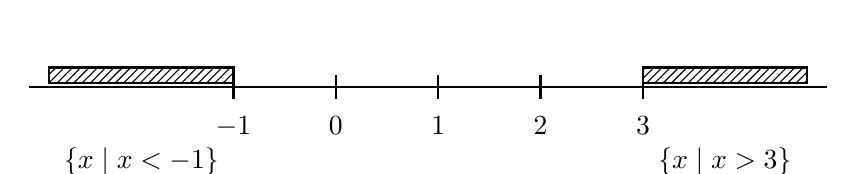
\begin{tikzpicture}[x=1.3cm, y=1cm]
    % Axis
    \draw[thick] (-3, 0) -- (4.8, 0);
    \foreach \x in {-1, 0, 1, 2, 3} {
        \draw[thick] (\x, 0.15) -- (\x, -0.15);
        \node[below=3pt] at (\x, -0.15) {$\x$};
    }

    % Shaded/hatched regions
    % x < -1
    \fill[pattern=north east lines, pattern color=black] (-2.8, 0.05) rectangle (-1, 0.25);
    \draw[thick] (-2.8, 0.05) rectangle (-1, 0.25);
    \node[below=14pt] at (-1.9, -0.15) {$\{x \mid x < -1\}$};

    % x > 3
    \fill[pattern=north east lines, pattern color=black] (3, 0.05) rectangle (4.6, 0.25);
    \draw[thick] (3, 0.05) rectangle (4.6, 0.25);
    \node[below=14pt] at (3.8, -0.15) {$\{x \mid x > 3\}$};
\end{tikzpicture}
\end{figure}

故（上）式的解是：$\{x \mid -1<x<3\}\cup\phi = \{x \mid -1<x<3\}$.

換句話說，坐標滿足原不等式的點在下圖所示 $A, B$ 間的點集內.

\begin{figure}[H]
\centering
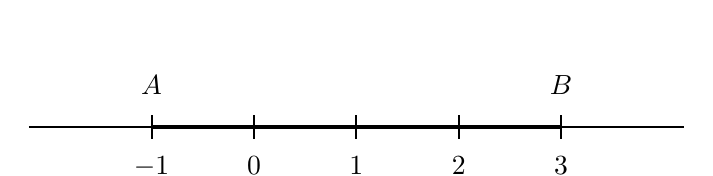
\begin{tikzpicture}[x=1.3cm, y=1cm]
    % Axis
    \draw[thick] (-2.2, 0) -- (4.2, 0);
    \foreach \x in {-1, 0, 1, 2, 3} {
        \draw[thick] (\x, 0.15) -- (\x, -0.15);
        \node[below=3pt] at (\x, -0.15) {$\x$};
    }

    % Segment AB
    \draw[ultra thick] (-1, 0) -- (3, 0);
    \node[above=4pt] at (-1, 0.15) {$A$};
    \node[above=4pt] at (3, 0.15) {$B$};
\end{tikzpicture}
\end{figure}

\begin{example}\label{ex:b2_2-3-3}
求直線上的點集，其坐標滿足下列不等式：
\[
f(x)=(x+1)(x-1)(x-3)>0.
\]
\end{example}

\noindent\textbf{【解】} 由符號定則，我們可以把上述不等方歸於
\[
x+1,\quad x-1,\quad x-3.
\]
這三個因子各種可能的正、負組合的討論. 同學們容易看出 $-1,\ +1,\ +3$ 分別是 $x+1,\ x-1$ 和 $x-3$ 這三個因子正、負的分界線. 今列表如下：

\begin{figure}[H]
\centering
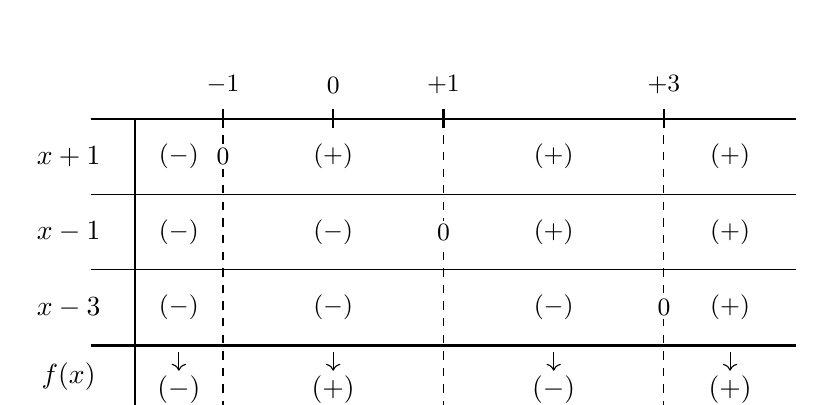
\begin{tikzpicture}[x=1.4cm, y=0.8cm]
    % Top number line
    \draw[thick] (-2.2, 3.5) -- (4.2, 3.5);
    \foreach \x/\label in {-1/-1, 0/0, 1/+1, 3/+3} {
        \draw[thick] (\x, 3.65) -- (\x, 3.35);
        \node[above=2pt] at (\x, 3.65) {\small $\label$};
    }

    % Vertical boundary lines (dashed)
    \draw[dashed] (-1, 3.5) -- (-1, -1.2);
    \draw[dashed] (1, 3.5) -- (1, -1.2);
    \draw[dashed] (3, 3.5) -- (3, -1.2);

    % Left border line
    \draw[thick] (-1.8, 3.5) -- (-1.8, -1.2);

    % Horizontal grid lines
    \draw[thin] (-2.2, 2.3) -- (4.2, 2.3);
    \draw[thin] (-2.2, 1.1) -- (4.2, 1.1);
    \draw[thick] (-2.2, -0.1) -- (4.2, -0.1);

    % Row 1: x+1
    \node at (-2.4, 2.9) {$x+1$};
    \node at (-1.4, 2.9) {\small $(-)$};
    \node at (-1, 2.9) [fill=white, inner sep=1pt] {\small $0$};
    \node at (0, 2.9) {\small $(+)$};
    \node at (2, 2.9) {\small $(+)$};
    \node at (3.6, 2.9) {\small $(+)$};

    % Row 2: x-1
    \node at (-2.4, 1.7) {$x-1$};
    \node at (-1.4, 1.7) {\small $(-)$};
    \node at (0, 1.7) {\small $(-)$};
    \node at (1, 1.7) [fill=white, inner sep=1pt] {\small $0$};
    \node at (2, 1.7) {\small $(+)$};
    \node at (3.6, 1.7) {\small $(+)$};

    % Row 3: x-3
    \node at (-2.4, 0.5) {$x-3$};
    \node at (-1.4, 0.5) {\small $(-)$};
    \node at (0, 0.5) {\small $(-)$};
    \node at (2, 0.5) {\small $(-)$};
    \node at (3, 0.5) [fill=white, inner sep=1pt] {\small $0$};
    \node at (3.6, 0.5) {\small $(+)$};

    % Row 4: f(x)
    \node at (-2.4, -0.6) {$f(x)$};
    \draw[->] (-1.4, -0.2) -- (-1.4, -0.5);
    \node at (-1.4, -0.8) {$(-)$};

    \draw[->] (0, -0.2) -- (0, -0.5);
    \node at (0, -0.8) {$(+)$};

    \draw[->] (2, -0.2) -- (2, -0.5);
    \node at (2, -0.8) {$(-)$};

    \draw[->] (3.6, -0.2) -- (3.6, -0.5);
    \node at (3.6, -0.8) {$(+)$};
\end{tikzpicture}
\end{figure}

由上述表格，我們可以一目瞭然地看出 $f(x)>0$ 的解是
\[
-1x<1\text{，及 } x>3.\phantomsection\label{note:b2-ch2-p37-ex3-typo}
\]

\begin{example}\label{ex:b2_2-3-4}
求解 $2x^2-6x+25<0$.
\end{example}

\noindent\textbf{【解】} 由於二次式 $2x^2-6x+25$ 的判別式
\[
\delta = (-6)^2 - 4\cdot 2\cdot 25 = -164 < 0,
\]
故由第一章的定理 3 的推論得知 $2x^2-6x+25$ 永遠為正，所以無解.

（同理：$2x^2-6x+25>0$ 的解是全部實數的集合）

\begin{example}\label{ex:b2_2-3-5}
求解不等式
\[
(2x^2-6x+25)(x+1)(x-1)(x-3)\le 0.
\]
\end{example}

\noindent\textbf{【解】} 由〔例 4〕的討論，$2x^2-6x+25$ 永遠是正的，所以
\begin{align*}
&(2x^2-6x+25)(x+1)(x-1)(x-3)\le 0, \\
&\Updownarrow \\
&(x+1)(x-1)(x-3)\le 0.
\end{align*}
仿照〔例 3〕的辦法列表解得
\[
x\le -1\text{，及 } 1\le x\le 3.
\]
（同理：$(-2x^2+6x-25)g(x)\ge 0$ 和 $g(x)\le 0$ 有同解，因為 $-2x^2+6x-25$ 永遠是負的.）

\begin{example}\label{ex:b2_2-3-6}
求解不等式
\[
f(x) = \frac{x+1}{(x-1)(x-3)} > 0.
\]
\end{example}

\noindent\textbf{【解】} 我們知道 $f(x)>0$ 的條件是要負的因子是偶數個，組成這個 $f(x)$ 的因子是 $x+1,\ x-1,\ x-3$，與〔例 3〕沒有什麼不一樣（只是 $x-1,\ x-3$ 被移到分母上罷了！）所以正負界限的討論，當然也應跟〔例 3〕相同. 那麼，什麼是 $f(x)>0$ 的解呢？自然也是：$-1<x<1,\ x>3$.

\subsubsection*{習題 2-3}

\begin{enumerate}
    \item 試以圖表示下列各組不等式的界限：
    \begin{enumerate}[(i)]
        \item $\begin{cases} x>-1 \\ x>2 \end{cases}$
        \item $\begin{cases} x>5 \\ x<7 \end{cases}$
        \item $\begin{cases} x<0 \\ x\le 2 \end{cases}$
        \item $\begin{cases} -1\le x\le 1 \\ x\ge -2 \\ -5<x<9 \end{cases}$
    \end{enumerate}

    \item 在直線上分別描出坐標，滿足下列不等式的點集：
    \begin{enumerate}[(i)]
        \item $\frac{x}{x+1}<0$.
        \item $\frac{(x-1)^2}{2x-1}<0$.
        \item $\frac{(x+1)(x+2)}{x+3}>0$.
        \item $\frac{x+1}{(x-1)(x-3)}\ge 0$.
    \end{enumerate}

    \item 分別求出直線上的點集，其坐標滿足下列不等式：
    \begin{enumerate}[(i)]
        \item $2x^2+4x>x^2+6x+8$.
        \item $(x+1)(x-3)(x-4)\le 0$.
        \item $|x-1|<3$.
        \item $x^2+2x+5>0$.
        \item $1<|3x+2|\le 7$.
    \end{enumerate}

    \item 試解下列不等式：
    \begin{enumerate}[(i)]
        \item $\frac{x^2-7x+12}{x^2-3x+2} < -1$.
        \item $\frac{4x^2-20x+18}{x^2-5x+4} < 3$.
        \item $\frac{1}{x+1}+\frac{1}{x+4} > \frac{1}{x+3}+\frac{1}{x+2}$.
    \end{enumerate}

    \item 證明
    \begin{enumerate}[(i)]
        \item 不等式 $1+x+x^2>0$ 對於所有實數 $x$ 都成立，一般地，不等式 $1+x+x^2+\dots+x^{2n}>0$ ($n$ 是自然數) 對於所有實數也都成立.
        \item 方程式 $x^{2n+1}-1=0$ 祗有一個實根 ($=1$).
    \end{enumerate}
\end{enumerate}

\subsection{數列的觀念與例子}\label{sec:b2_2-4}

首先，讓我們再來看看我們在數學領域中最先認識的老朋友——自然數.
\[
1, 2, 3, 4, 5, \dots, n, n+1, n+2, \dots.
\]
他們是一串依次排列的數，從 1 開始，逐次加以 1 至無窮. 這就是本節要向大家介紹的數列（sequence）的一個原始的例子. 在正式定義數列之前，讓我們再來舉幾個數列的例子.

\begin{example}\label{ex:b2_2-4-1}
假如你從今天開始每天儲蓄 10 元，則第一天你儲了 10 元，第二天你共儲了 20 元，以此類推，到第 $n$ 天共儲有 $10\cdot n$ 元. 所以，你在各天儲蓄的累積總額可寫成下述數列.
\[
10, 20, 30, 40, \dots, n\cdot 10, (n+1)\cdot 10 \dots\dots
\]
\end{example}

\begin{example}\label{ex:b2_2-4-2}
假如你不但每天儲蓄 10 元，而且每儲滿 100 元時，就存入銀行，因而多得千分之一的日利（假設用單利法），那麼你每天的儲蓄累積總額就是下述數列：
\[
10, 20, 30, \dots, 90, 100;\ 110.1, 120.2, \dots, 201;\ 211.2, 221.4, \dots, 303;\ \dots
\]
以此類推，請同學試求上述數列的第 $365, 730, 1096, 1461$ 項.
\end{example}

\subsubsection*{4-1 數列的定義}

一個數列就是一串（如自然數一般）依次排列的數.

\begin{example}\label{ex:b2_2-4-3}
\leavevmode
\begin{enumerate}[(i)]
    \item $1, -1, 1, -1, \dots, (-1)^n, \dots$ 為一數列，其第 $n+1$ 項為 $(-1)^n$.
    \item $1, 0, -1, 0, 1, 0, -1, \dots$ 為一數列，其偶數項為 0，第 $4k+1$ 項為 1，第 $4k+3$ 項為 $-1$.
    \item $1, 4, 9, 16, \dots, n^2, \dots$ 為一數列，其第 $n$ 項為 $n^2$.
    \item $2, 3, 5, 7, 11, 13, \dots$, 第 $n$ 個質數, $\dots$ 為一數列，（因為在第一冊第六章中證明質數個數無窮.）
    \item $1, -1, 3, 7, 0, 0, \dots, 0, \dots$ 為一數列它的前四項為 $1, -1, 3, 7$，而自第五項起，皆為 0.
    \item $0, 0, 1, 0, 0, -1;\ 0, 0, 2, 0, 0, -2, \dots;\ 0, 0, n, 0, 0, -n+1, 0, 0, -(n+1), \dots$\phantomsection\label{note:b2-ch2-p40-ex3-vi} 為一數列，其第 $6n$ 項為 $-n$，第 $6n-3$ 項為 $n$，其他各項為零.
    \item $1, \frac{1}{2}, \frac{1}{3}, \frac{1}{4}, \dots, \frac{1}{n}, \dots$ 是第 $n$ 項為 $\frac{1}{n}$ 的數列.
    \item $a, a^2, a^3, \dots, a^n, \dots$ 是第 $n$ 項為 $a^n$ 的數列.
    \item $1, 4, 1, 5, 9, 2, 6, \dots$, （第 $n$ 項是 $\pi=3.1415926\dots$ 小數點線下的第 $n$ 位數字）.
\end{enumerate}
\end{example}

\subsubsection*{4-2 關於數列的符號用法}

在今後對於數列的討論中，我們將用 $a_n, b_n$ 或 $S_n, \dots$ 等符號表示某給定數列的第 $n$ 項（亦即用足標去標明第幾項）. 用符號
\[
\langle a_n \mid n=1, 2, 3, \dots \rangle \quad (\text{或簡寫成 } \langle a_n \rangle)
\]
去表示第 $n$ 項為 $a_n$ 的數列. 例如：$\langle (-1)^n \mid n=1, 2, 3, \dots \rangle$ 就是數列 $-1, +1, -1, +1, \dots$,
\[
\langle \frac{1}{1+n^2} \rangle \text{ 就是數列 } \frac{1}{2}, \frac{1}{5}, \frac{1}{10}, \frac{1}{17}, \dots
\]

\subsubsection*{4-3 數列的種類及其定義}

我們常見的數列例子有等差數列與等比數列

\begin{definition*}
等差數列 $\langle a_n \rangle$ 就是滿足 $a_2-a_1 = a_3-a_2 = a_n-a_{n-1} = \dots = d$ 的數列，$a_1$ 叫做首項，$d$ 叫做公差.
\end{definition*}

\begin{definition*}
等比數列（或幾何數列）$\langle b_n \rangle$ 就是滿足 $\frac{b_2}{b_1} = \frac{b_3}{b_2} = \dots = \frac{b_n}{b_{n-1}} = \dots = r$ 的數列（設各項 $\ne 0$）. $b_1$ 叫做首項，$r$ 叫做公比.
\end{definition*}

我們甚至可以用等差數列來做出一種新的數列：如果 $\langle a_n \rangle$ 為一等差數列，每一項 $a_n \ne 0$，我們就把 $a_n$ 的倒數所成的數列 $\langle \frac{1}{a_n} \rangle$ 叫做調和數列. 也就是說我們有：

\begin{definition*}
調和數列 $\langle h_n \rangle$ 就是滿足
\[
\frac{1}{h_2}-\frac{1}{h_1} = \frac{1}{h_3}-\frac{1}{h_2} = \dots = \frac{1}{h_n}-\frac{1}{h_{n-1}}
\]
的數列.
\end{definition*}

顯然地，$\frac{2}{h_2} = \frac{1}{h_1}+\frac{1}{h_3} = \frac{h_1+h_3}{h_1 h_3}$， $2h_1 h_3 = h_2(h_1+h_3)$.

所以一般相連的項之間有下列關係：
\[
2h_{n-1}h_{n+1} = h_n(h_{n-1}+h_{n+1}).
\]

\subsubsection*{習題 2-4}

\begin{enumerate}
    \item 已知等比數列中兩項，求數列的前五項及一般項 $a_n$：
    \begin{enumerate}[(i)]
        \item $a_2=\frac{121}{100},\ a_4=\frac{1331}{1000}$.
        \item $b_2=6,\ b_5=48$.
        \item $c_6=18,\ c_9=54$.
        \item $d_4=\frac{4}{9},\ d_7=\frac{32}{243}$.
    \end{enumerate}

    \item 已知等差數列中某二項，求數列的前五項及一般項 $a_n$：
    \begin{enumerate}[(i)]
        \item $a_3=5,\ a_8=9$.
        \item $a_4=10,\ a_{11}=6$.
        \item $a_9=30$, 公差 $=-5$.
    \end{enumerate}

    \item 如果 $\langle a_n \rangle$ 是一個等比數列，證明 $\langle \frac{1}{a_n} \rangle$ 也是一個等比數列.

    \item 已知調和數列兩項，求前五項及一般項 $a_n$：
    \begin{enumerate}[(i)]
        \item 第三項是 3，第七項是 3.
        \item 第二項是 $\frac{1}{9}$，第十一項是 $\frac{1}{50}$.
    \end{enumerate}
\end{enumerate}

\subsection{極限的概念及基本性質}\label{sec:b2_2-5}

數列在數學中的重要性在於它是討論極限的基本工具. 本節將對數列的極限及其基本性質作一初步介紹. 在下一章中，我們將進一步用它來討論實數系的重要特性——完備性（或稱為連續性）. 極限概念和實數系的完備性是往後微積分學的基礎，也是研究自然現象、工程問題、統計學等等所不可或缺的基本工具.

\subsubsection*{5-1 極限概念}

\begin{example}\label{ex:b2_2-5-1}
仔細觀察數列 $1, \frac{1}{2}, \frac{1}{3}, \frac{1}{4}, \dots, \frac{1}{n}, \dots$，我們馬上看出：
\begin{enumerate}[(i)]
    \item 上述數列的每項都是正數.
    \item 上述數列，逐項遞減：
    \[
    1 > \frac{1}{2} > \frac{1}{3} > \dots > \frac{1}{n} > \frac{1}{n+1} > \dots.
    \]
    \item 當 $n$ 愈來愈大時，第 $n$ 項 $\frac{1}{n}$ 不但愈來愈接近 0，而且要多近就能多近. 這種情形，我們就說：數列 $\langle \frac{1}{n} \rangle$ 趨近 0，或收斂到 0，或 0 是數列 $\langle \frac{1}{n} \rangle$ 的極限，用記號
    \[
    \frac{1}{n}\to 0, \quad \text{或 } \lim_{n\to\infty}\frac{1}{n}=0, \quad \text{或 } \lim\frac{1}{n}=0 \text{ 表示}.
    \]
\end{enumerate}
\end{example}

現在讓我們再用直線坐標系，把上述事實圖解說明如下：

\begin{figure}[H]
\centering
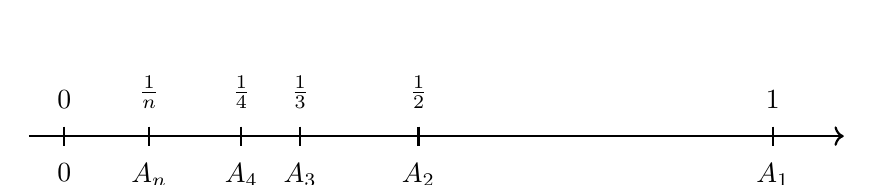
\begin{tikzpicture}[x=9cm, y=1cm]
    % Number line
    \draw[thick, ->] (-0.05, 0) -- (1.1, 0);

    % Ticks and coordinates
    % 0
    \draw[thick] (0, 0.12) -- (0, -0.12);
    \node[above=3pt] at (0, 0.12) {$0$};
    \node[below=3pt] at (0, -0.12) {$0$};

    % 1/n
    \draw[thick] (0.12, 0.12) -- (0.12, -0.12);
    \node[above=3pt] at (0.12, 0.12) {$\frac{1}{n}$};
    \node[below=3pt] at (0.12, -0.12) {$A_n$};

    % 1/4
    \draw[thick] (0.25, 0.12) -- (0.25, -0.12);
    \node[above=3pt] at (0.25, 0.12) {$\frac{1}{4}$};
    \node[below=3pt] at (0.25, -0.12) {$A_4$};

    % 1/3
    \draw[thick] (0.333, 0.12) -- (0.333, -0.12);
    \node[above=3pt] at (0.333, 0.12) {$\frac{1}{3}$};
    \node[below=3pt] at (0.333, -0.12) {$A_3$};

    % 1/2
    \draw[thick] (0.5, 0.12) -- (0.5, -0.12);
    \node[above=3pt] at (0.5, 0.12) {$\frac{1}{2}$};
    \node[below=3pt] at (0.5, -0.12) {$A_2$};

    % 1
    \draw[thick] (1.0, 0.12) -- (1.0, -0.12);
    \node[above=3pt] at (1.0, 0.12) {$1$};
    \node[below=3pt] at (1.0, -0.12) {$A_1$};
\end{tikzpicture}
\end{figure}

在直線上取以數列：
\[
1, \frac{1}{2}, \frac{1}{3}, \frac{1}{4}, \dots, \frac{1}{n}, \dots
\]
的各項為坐標的各點，就得到一個點列：
\[
A_1, A_2, A_3, \dots, A_n, \dots.
\]
上述點列 $\langle A_n \rangle$ 從原點 0 的右邊逐步向原點逼近：
\[
0 < \dots < A_{n+1} < A_n < \dots < A_3 < A_2 < A_1;
\]
而且可以逼近到隨心所欲的程度.

\begin{example}\label{ex:b2_2-5-2}
$\frac{1}{2}, \frac{2}{3}, \frac{3}{4}, \dots, \frac{n}{n+1}, \dots$
\end{example}
同學們可以容易看出這個數列逐項遞增，其第 $n$ 項 $a_n = \frac{n}{n+1}$ 永遠小於 1，但是當 $n$ 愈來愈大時，$a_n$ 和 1 的差異 $|a_n-1| = \frac{1}{n+1}$ 可以小到隨心所欲的小. 換句話說，
\[
\frac{n}{n+1} \to 1.
\]

\begin{example}\label{ex:b2_2-5-3}
$(-\frac{1}{2}), (-\frac{1}{2})^2, (-\frac{1}{2})^3, (-\frac{1}{2})^4, \dots, (-\frac{1}{2})^n, \dots$
\end{example}
這個數列逐項正負相間，所以不再是遞減或遞增數列，但是其第 $n$ 項 $a_n$ 和 0 的差異 $|a_n-0| = |a_n| = (\frac{1}{2})^n$ 顯然可以小到隨心所欲的小. 所以
\[
\lim\left(-\frac{1}{2}\right)^n = 0
\]

以上三個例子的數列，都有極限，這樣的數列叫做收斂數列. 但是並不是每一個數列都收斂；不收斂的數列叫做發散數列. 請看下例：

\begin{example}\label{ex:b2_2-5-4}
數列 $1, 4, 9, 16, \dots, n^2, \dots$ 顯然沒有極限.
\end{example}

\begin{example}\label{ex:b2_2-5-5}
數列 $+1, -1, +1, -1, +1, \dots$ 也不收斂.
\end{example}

\paragraph{註：} 例 4 的情形為發散至正無窮大，寫做 $n^2 \to \infty$. 例 5 的情形叫做振動. 當然還有其他發散的情形. 例如數列 $1, -2, +3, -4, +5, \dots$.

\begin{example}\label{ex:b2_2-5-6}
級數 $1, r, r^2, r^3, r^4, \dots, r^n, \dots$\phantomsection\label{note:b2-ch2-p44-ex6-series-term} 的收斂與發散有下列幾種情形：
\begin{align*}
&\text{當 } r<1 \text{ 時 } \lim_{n\to\infty} r^n = 0\phantomsection\label{note:b2-ch2-p44-ex6-r-range} \\
&\text{當 } r=1 \text{ 時 } \lim_{n\to\infty} r^n = 1 \\
&\text{當 } r>1 \text{ 時 } \lim_{n\to\infty} r^n = \infty
\end{align*}
\end{example}

\subsubsection*{習題 2-5}

\begin{enumerate}
    \item 問下列數列是收斂？還是發散？
    \begin{enumerate}[(i)]
        \item $1, -0.2, 0.04, -0.008, \dots$, 第 $n$ 項為 $(\frac{-2}{10})^{n-1}$.
        \item $3, \frac{3}{2}, \frac{3}{4}, \frac{3}{8}, \dots$ 第 $n$ 項為 $\frac{3}{2^{n-1}}$.
        \item $10, \frac{10^2}{9}, \frac{10^3}{9^2}, \dots$, 第 $n$ 項為 $\frac{10^n}{9^{n-1}}$.
    \end{enumerate}

    \item 下列數列中那些是收斂？那些是發散到 $\infty$？
    \begin{enumerate}[(i)]
        \item $a_n = n^2$.
        \item $a_n = \frac{100\cdot n}{n^2}$.
        \item $a_n = \frac{n^2-1}{n+100}$.
        \item $a_n = \frac{1-n}{1+n}$.
        \item $a_n = (-1)^n n$.
    \end{enumerate}

    \item 證明
    \begin{enumerate}[(i)]
        \item 如果等差數列 $\langle a_n \rangle$ 的公差 $>0$，那麼 $\langle a_n \rangle$ 是遞增數列；反之如果公差 $<0$ 就是遞減數列.
        \item 如果等比數列 $\langle a_n \rangle$ 的公比 $r>1$，那麼 $\langle a_n \rangle$ 是遞增數列. 反之如果 $0<r<1$ 就是遞減.
        \item 調和數列不是遞增就是遞減數列.
    \end{enumerate}
\end{enumerate}

\subsubsection*{5-2 極限的基本性質}

如果兩個數列 $\langle a_n \rangle$、$\langle b_n \rangle$ 都收斂，那麼它們的和數列 $\langle a_n+b_n \rangle$、差數列 $\langle a_n-b_n \rangle$、積數列 $\langle a_n b_n \rangle$ 也都收斂，而且有
\begin{enumerate}[(i)]
    \item $\lim(a_n+b_n) = \lim a_n + \lim b_n$.
    \item $\lim(a_n-b_n) = \lim a_n - \lim b_n$.
    \item $\lim a_n b_n = \lim a_n \cdot \lim b_n$.
\end{enumerate}

\begin{example}\label{ex:b2_2-5-7}
常數數列 $c, c, c, \dots, c, \dots$ 當然收斂到 $c$.
\end{example}

\begin{example}\label{ex:b2_2-5-8}
由例 7 及性質 (iii) 就得：如果 $\langle a_n \rangle$ 收斂，那麼
\[
\lim c a_n = c \lim a_n.
\]
\end{example}

轉到商數列 $\langle \frac{a_n}{b_n} \rangle$ 的討論，大家當然要問：如果數列 $\langle a_n \rangle$，$\langle b_n \rangle$ 收斂，是不是商數列 $\langle \frac{a_n}{b_n} \rangle$ 也收斂？收斂到 $\frac{\lim a_n}{\lim b_n}$？

當然 $b_n$ 都不能等於 0，不然的話商數列 $\langle \frac{a_n}{b_n} \rangle$ 就沒有意義，同樣的道理 $\lim b_n$ 也不能是 0，不然的話 $\frac{\lim a_n}{\lim b_n}$ 也沒有意義. 事實上，這個必要條件也是充分條件.

如果 $\langle a_n \rangle$，$\langle b_n \rangle$ 都收斂，而且 $b_n$ 都不等於 0，以及 $\lim b_n \ne 0$，那麼商數列 $\langle \frac{a_n}{b_n} \rangle$ 收斂，而且
\begin{enumerate}[(iv)]
    \item $\lim\frac{a_n}{b_n} = \frac{\lim a_n}{\lim b_n}$.
\end{enumerate}

\begin{example}\label{ex:b2_2-5-9}
數列 $\langle \frac{1}{n^2} \rangle$，$\langle \frac{1}{n} \rangle$ 都收斂到 0，但商數列
\[
\langle \frac{\frac{1}{n^2}}{\frac{1}{n}} \rangle = \langle \frac{1}{n} \rangle \text{ 收斂到 0，但 } \langle \frac{\frac{1}{n}}{\frac{1}{n^2}} \rangle = \langle n \rangle \text{ 發散到無窮大}.
\]
所以 $\lim b_n = 0$ 時，商數列 $\langle \frac{a_n}{b_n} \rangle$ 可能收斂也可能發散.
\end{example}

\subsubsection*{習題 2-6}

\begin{enumerate}
    \item 求下列各數列之極限：
    \begin{enumerate}[(i)]
        \item $\overbrace{0, 0, 0, 0, \dots, 0}^{1000\text{項}}, 1, 1, 1, \dots, 1, \dots$ （即前 1000 項都是 0，以後都是 1）.
        \item $0, 0, 0, 0, \dots, 0\dots$ （每一項都是 0）.
        \item $(6+\frac{1}{n})(\frac{n+2}{2n+1}-1)$.
        \item $(\frac{2n^2-3}{3n^2-2})^2$.
        \item $\frac{n^2+n+1}{\frac{n^2+3}{n+1}}$.
        \item $3n(\frac{2}{n}+\frac{2n^2+9}{n^3+n+1.5})$.
        \item $\frac{2n^2(n-3+4n^2)}{5(n-1)^3(3n+4)}$.
    \end{enumerate}

    \item 設 $a_n = \frac{2n+1}{n^2},\ b_n = \frac{1-n^2}{3+n-n^2},\ c_n = \frac{n^3}{1-n}$，求下列各數列之極限：
    \[
    \langle a_n \rangle,\quad \langle b_n \rangle,\quad \langle c_n \rangle,\quad \langle a_n+c_n \rangle,\quad \langle b_n c_n \rangle,\quad \langle \frac{a_n}{c_n} \rangle,\quad \langle \frac{c_n}{a_n} \rangle,
    \]
    \[
    \langle -\frac{b_n}{c_n} \rangle,\quad \langle \frac{b_n}{a_n} \rangle,\quad \langle 3a_n - \frac{1}{2}b_n \rangle,\quad \langle \frac{4b_n}{a_n+c_n} \rangle.
    \]

    \item 求下列各極限：
    \begin{enumerate}[(i)]
        \item $\lim_{n\to\infty}(\frac{n^2-n}{n+1}-\frac{n^2+n}{n-1})$.
        \item $\lim_{n\to\infty}(\frac{101}{100})^n$.
        \item $\lim_{n\to\infty}(\frac{99}{100})^n$.
    \end{enumerate}
\end{enumerate}

\subsection{無窮級數和循環小數}\label{sec:b2_2-6}

小學和中學都教過：循環小數
\[
0.6666\dots = \frac{2}{3}.
\]
在這一節中我們要仔細思考它的意思，證明每個循環小數都等於一個分數，而每個分數都等於一個循環小數.

\subsubsection*{6-1 無限小數}

從整數因子分解的唯一性，我們得知：一個不可約分數 $\frac{p}{q}$ ($p, q$ 互質) 能表成一個有限位小數的必要充分條件是 $q$ 只含有 2 或 5 這兩種質因子. 譬如 $\frac{2}{3}, \frac{5}{7}$ 等分數不能表成有限小數. 今以 $\frac{2}{3}$ 為例，作下述分析：

\begin{enumerate}[(i)]
    \item 以 3 去除 2，得
    \[
    \begin{array}{r@{\quad}l}
        & 0.666\dots \\
        \cline{2-2}
        3 & )\, 2000\dots \\
        & \phantom{)\, 1} 18 \\
        \cline{2-2}
        & \phantom{)\, 0} 20 \\
        & \phantom{)\, 0} 18 \\
        \cline{2-2}
        & \phantom{)\, 00} 20 \\
        & \phantom{)\, 00} 18 \\
        \cline{2-2}
        & \phantom{)\, 000} 2
    \end{array}
    \]

    \item 上述除式的意義是：
    \begin{align*}
    2 = 0.6\times 3 + 0.2 &\iff 0.6 < \frac{2}{3} < 0.7, \\
    = 0.66\times 3 + 0.02 &\iff 0.66 < \frac{2}{3} < 0.67, \\
    = 0.666\times 3 + 0.002 &\iff 0.666 < \frac{2}{3} < 0.667, \\
    &\dots\dots\dots\dots\dots\dots\dots
    \end{align*}
\end{enumerate}

從上面的分析，同學們可以看出 $\frac{2}{3}$ 雖然不能用有限位小數表出，但是存在着由有限位小數所成的數列：
\[
a_1 = 0.6,\quad a_2 = 0.66,\quad a_3 = 0.666\dots,\quad a_n = \underbrace{0.666\dots 66}_{n\text{ 位小數}}
\]
上述數列和 $\frac{2}{3}$ 的關係是
\[
a_n = \underbrace{0.666\dots 66}_{n\text{ 位}} < \frac{2}{3} < \underbrace{0.666\dots 67}_{n\text{ 位}} = a_n + \frac{1}{10^n}.
\]
換句話說，$a_n$ 和 $\frac{2}{3}$ 之間的差異小於 $\frac{1}{10^n}$，這個差異當 $n$ 越來越大時，當然會任意地小. 所以
\[
a_n \to \frac{2}{3}
\]
我們通常寫 $0.666\dots = \frac{2}{3}$ 的意思就是這樣：如果
\[
a_n = \underbrace{0.666\dots 66}_{n\text{ 位}},
\]
那麼
\[
a_n \to \frac{2}{3}.
\]
同樣地，我們寫 $\pi = 3.1415926\dots$ 時，我們的意思是：

令 $a_1=3.1,\ a_2=3.14,\ a_3=3.141,\ a_4=3.1415,\ \dots$

那麼 $a_n \to \pi$.

若把 \hyperref[sec:b2_2-4]{§ 4}〔例 3〕之 (ix) 的數列寫做 $c_n$，那麼
\[
a_n = 3 + \sum_{k=1}^n \frac{c_k}{10^k}.
\]
所以無限小數的解釋是這個樣子：我們取它小數點以下第 $n$ 位為止的有限小數，記做 $a_n$，那麼數列 $a_n$ 的極限就等於這個無限小數.

讓我們回憶一下從前怎樣證明 $0.6666\dots = \frac{2}{3}$，根據以上的解釋，這個式子表示 $a_n \to \frac{2}{3}$，其中
\[
a_n = \underbrace{0.666\dots 66}_{n\text{ 位}}.
\]
我們說：因為
\[
a = 0.666\dots
\]
所以
\[
10a = 6.666\dots
\]
所以
\[
9a = 10a-a = 6,\quad \text{即 } a = \frac{6}{9} = \frac{2}{3}.
\]
這個論證其實稍微有點問題：因為你必須先假定 $a=0.666\dots$ 這個數的存在（也就是說 $a_n$ 收斂）. 這一點參看下一章，不過我們有另一個辦法，不需這個假定.

我們看出 $a_n$ 和 $a_{n-1}$ 的差是 $\underbrace{0.000\dots 0}_{n\text{ 位}}6$. 這個差越來越小，而且“每步就小 10 倍”. 換句話說
\begin{align*}
a_1 &= 0.6 = b_1; \\
a_2 &= 0.6+0.06 = b_1+b_2,\quad \text{其中 } b_2 = b_1 \frac{1}{10}; \\
a_3 &= 0.6+0.06+0.006 = b_1+b_2+b_3,\quad \text{其中 } b_3 = b_2 \frac{1}{10};
\end{align*}
依此類推，而有
\[
a_n = b_1+b_2+b_3+\dots+b_n,
\]
其中 $b_1 = 0.6$，而 $b_n = b_1 r^{n-1},\ r = \frac{1}{10}$.

當我們看差額 $a_n - a_{n-1} = b_n$ 時，我們就有一個無窮等比數列 $\langle b_n \rangle$. $a_n$ 是這數列的首 $n$ 項和. 而我們想去證明的也就是
\[
b_1+b_2+b_3+\dots = \frac{2}{3}.
\]
(即 $\sum_{i=1}^n b_i \to \frac{2}{3}$)

我們利用眾所週知的公式：
\[
(1-r)(1+r+r^2+\dots+r^{k-1}) = 1-r^k
\]
因此當 $r\ne 1$ 時，有
\[
1+r+r^2+\dots+r^{k-1} = \frac{1-r^k}{1-r}.
\]
可以知道
\begin{equation}\label{eq:b2_ch2_geom_sum}
b_1+b_1 r+b_1 r^2+\dots+b_1 r^{n-1} = b_1 \frac{1-r^n}{1-r} = \frac{b_1}{1-r} + \frac{-r^n}{1-r} \dots\dots(1)
\end{equation}
\phantomsection\label{note:b2-ch2-p50-eq1-b1}

在我們的例子，$|r|<1$，因此由（5-1）〔例 6〕$\frac{-r^n}{1-r} \to 0$\phantomsection\label{note:b2-ch2-p51-lim-rn}，所以
\[
a_n = b_1+b_1 r+b_1 r^2+\dots+b_1 r^{n-1} \to \frac{b_1}{1-r}, \quad (|r|<1).
\]
我們就寫成
\begin{equation}\label{eq:b2_ch2_geom_series_23}
\frac{2}{3} = \sum_{i=0}^\infty b_1 r^i = \frac{b_1}{1-r},\quad (|r|<1) \dots\dots(2)
\end{equation}
的形式.

\subsubsection*{6-2 無窮級數}

上面的證明也提示了一些新的概念：（無窮）級數.

一般的來說，如果 $\langle b_n \rangle$ 是個數列，那麼我們用記號
\[
b_1+b_2+b_3+\dots \quad \text{或} \quad \sum_{i=1}^\infty b_i
\]
表示一個級數.

我們把首 $n$ 項的和
\[
a_n = b_1+b_2+\dots+b_n
\]
叫做第 $n$ 個部分和. 這種部分和所成的數列 $\langle a_n \rangle$ 如果收斂，那麼我們說這級數 $\sum_{n=1}^\infty b_n$ 收斂，並且把 $\lim_{n\to\infty} a_n$ 叫做這級數的和. 而記做
\[
\sum_{n=1}^\infty b_n = \lim_{n\to\infty} a_n.
\]
反之，如果 $\langle a_n \rangle$ 發散，我們就說級數 $\sum_1^\infty b_n$ 發散. $b_n$ 叫做級數 $\sum_1^\infty b_n$ 的第 $n$ 項，而當數列 $\langle b_n \rangle$ 是等比數列時，級數 $\sum_1^\infty b_n$ 叫等比級數.

數列 $\langle b_n \rangle$ 的公比就是級數 $\sum_1^\infty b_n$ 的公比. 為了討論循環小數及下一章的需要，讓我們來看看下面兩個定理：

\begin{theorem}\label{thm:b2_2-6-1}
如果 $\sum_{n=1}^\infty b_n$ 是等比級數，那麼它收斂的充分必要條件是公比 $r$ 的絕對值小於 1，此時它的和是 $\frac{b_1}{1-r}$.
\end{theorem}

\noindent\textbf{【證明】} 充分性，從 (1)、(2) 兩式馬上知道，要證明必要性，我們只須注意到，如果 $|r| \ge 1$，那麼 $b_n = b_1 r^{n-1}$ 不會趨近于 0，但我們顯然有下列定理

\begin{theorem}\label{thm:b2_2-6-2}
如果數列 $\langle a_n \rangle$ 收斂，那麼 $a_n - a_{n-1}$ 收斂到 0. 因此，如果級數 $\sum_{n=1}^\infty b_n$ 收斂，那麼 $b_n \to 0$，因為第 $n$ 部分和是 $a_n = \sum_{i=1}^n b_i$，所以 $a_n - a_{n-1} = b_n \to 0$.
\end{theorem}

\begin{example}\label{ex:b2_2-6-1}
$\frac{1}{1}+\frac{1}{2}+\frac{1}{3}+\dots+\frac{1}{n}+\dots$ 是發散級數. 為什麼呢？我們首先注意到這是正項級數，因此，部分和會越來越大. 而且
\begin{align*}
a_1 &= 1, \\
a_2 &= 1+\frac{1}{2}, \\
a_4 &= 1+\frac{1}{2}+\frac{1}{3}+\frac{1}{4} > 1+\frac{1}{2}+\frac{1}{4}+\frac{1}{4} = 1+\frac{1}{2}+\frac{1}{2}, \\
a_8 &= 1+\frac{1}{2}+\frac{1}{3}+\frac{1}{4}+\frac{1}{5}+\frac{1}{6}+\frac{1}{7}+\frac{1}{8} \\
&> 1+\frac{1}{2}+\frac{1}{4}+\frac{1}{4}+\frac{1}{8}+\frac{1}{8}+\frac{1}{8}+\frac{1}{8} = 1+\frac{1}{2}+\frac{1}{2}+\frac{1}{2}.
\end{align*}
一般地
\[
a_{2^m} > 1 + \underbrace{\frac{1}{2}+\frac{1}{2}+\dots+\frac{1}{2}}_{m\text{ 個}} = \frac{m+2}{2}
\]
因 $a_{2^m}$ 越來越大毫無止境！所以 $a_n$ 只有發散到無限大.

注意到：$b_n = \frac{1}{n} \to 0$. 因此，定理 2 中的 $b_n \to 0$ 是 $\sum b_n$ 收斂的必要條件，但並非充分條件.
\end{example}

\subsubsection*{習題 2-7}

\begin{enumerate}
    \item 求級數的和：
    \begin{enumerate}[(i)]
        \item $1 - \frac{1}{2} + \frac{1}{4} - \dots + (-\frac{1}{2})^{n-1} + \dots$.
        \item $\frac{1}{1\cdot 2} + \frac{1}{2\cdot 3} + \frac{1}{3\cdot 4} + \dots + \frac{1}{n\cdot(n+1)} + \dots$.
        
        （提示：$\frac{1}{n(n+1)} = \frac{1}{n} - \frac{1}{n+1}$）
        \item $3 + \frac{3}{8} + \dots + \frac{3}{8^{n-1}} + \dots$.
    \end{enumerate}

    \item 設一等差數列 $\langle a_n \rangle$ 的公差是 $d$，寫出其第 $n$ 項與前 $n$ 項和的公式.

    \item 有一等差數列 $\langle a_n \rangle$，首項 $a_1=3,\ a_{15}=-25$，求它的公差和前 15 項和.

    \item 證明無窮級數 $1 + \frac{1}{3} + \frac{1}{5} + \frac{1}{7} + \dots + \frac{1}{2n-1} + \dots$ 是發散的.

    \item 如果 $\langle a_n \rangle$ 是等差數列，證明級數
    \[
    a_1+a_2+\dots+a_n+\dots
    \]
    是發散級數.

    \item 已知級數的部分和，寫出各級數與它們的和：
    \begin{enumerate}[(i)]
        \item $S_n = \frac{1}{2^n}$.
        \item $S_n = 1 - \frac{1}{n}$.
        \item $S_n = \frac{7^{n-1}-1}{3\cdot 7^{n-2}}$.
    \end{enumerate}
\end{enumerate}

\subsubsection*{6-3 循環小數和分數}

下面定理 3 關於循環小數與分數間關係的證明，可能讀起來有些抽象. 所以我們先用例子來說明一下.

\begin{example}\label{ex:b2_2-6-2}
試將 $0.3\overline{12}\ (=0.3121212\dots)$ 化為分數.
\end{example}

\noindent\textbf{【解】} 
\begin{align*}
0.3\overline{12} &= \frac{3}{10}+\left(\frac{1}{10^2}+\frac{2}{10^3}\right)+\left(\frac{1}{10^4}+\frac{2}{10^5}\right)+\left(\frac{1}{10^6}+\frac{2}{10^7}\right)+\dots \\
&= \frac{3}{10}+\frac{12}{10^3}+\frac{12}{10^5}+\frac{12}{10^7}+\dots \\
&= \frac{3}{10}+\frac{12}{10^3}\left(1+\frac{1}{10^2}+\frac{1}{10^4}+\frac{1}{10^6}+\dots\right) \\
&= \frac{3}{10}+\frac{12}{10^3}\cdot\frac{1}{1-\frac{1}{10^2}} \\
&= \frac{3}{10}+\frac{12}{10^3}\cdot\frac{10^2}{99} \\
&= \frac{3}{10}+\frac{12}{990} \\
&= \frac{103}{330}.
\end{align*}
當我們仔細看這個例子，可以知道所以能夠將這個極限（也就是這個分數）找出來，是因為將第一個循環部分（就是 $\frac{12}{10^3}=0.012$）提出來後，在括弧內的級數是 $1+\frac{1}{10^2}+\frac{1}{10^4}+\dots+\frac{1}{10^{2n}}+\dots$ 這樣的等比級數. 它們的公比是 $\frac{1}{100}(<1)$，所以有極限 $\frac{100}{99}$，而由這個極限就可以逐步算出整個循環小數的極限了.

\begin{example}\label{ex:b2_2-6-3}
試將 $\frac{8}{33}$ 化為小數.
\end{example}

\noindent\textbf{【解】} 利用除法：
\[
\begin{array}{r@{\quad}ll}
    & 0.242424\dots & \\
    \cline{2-2}
    33 & )\, 80 & \\
    & \phantom{)\, } 66 & \\
    \cline{2-2}
    & \phantom{)\, } 140 & \left.\vphantom{\begin{array}{c}1\\1\end{array}}\right\} * \\
    & \phantom{)\, } 132 & \\
    \cline{2-2}
    & \phantom{)\, 0} 80 & \\
    & \phantom{)\, 0} 66 & \\
    \cline{2-2}
\end{array}
\]

我們由上面的除式看出，所以能每隔兩位就重複的緣故是 $*$ 部分相減後剩餘為 8，而開始也是 8，既然除數不變，那麼一切過程會再來一次，這樣一次一次的重複，就成了循環小數.

如果 $a$ 是個循環小數，它的循環節是由第 $k+1$ 位開始，到 $k+l$ 位. 平常我們寫做
\[
a = a_0.c_1 c_2 \dots c_k \overline{c_{k+1} c_{k+2} \dots c_{k+l}}.
\]
($c_i$ 及 $a_0$ 是整數，而 $0\le c_i < 10,\ 0\le a_0$)

它的意思就是
\begin{align*}
a = a_0 &+ \frac{c_1}{10} + \frac{c_2}{10^2} + \dots + \frac{c_k}{10^k} + \frac{c_{k+1}}{10^{k+1}} + \dots + \frac{c_{k+l}}{10^{k+l}} \\
&+ \frac{c_{k+1}}{10^{k+l+1}} + \frac{c_{k+2}}{10^{k+l+2}} + \dots + \frac{c_{k+l}}{10^{k+2l}} + \frac{c_{k+1}}{10^{k+2l+1}} + \dots
\end{align*}
顯然的，這不是個等比級數.

第 $k$ 個部分和是分數
\[
a_k = a_0 + \frac{c_1}{10^1} + \frac{c_2}{10^2} + \dots + \frac{c_k}{10^k}.
\]
如果我們令
\[
d \equiv \frac{c_{k+1}}{10^{k+1}} + \frac{c_{k+2}}{10^{k+2}} + \frac{c_{k+3}}{10^{k+3}} + \dots + \frac{c_{k+l}}{10^{k+l}}
\]
（所以 $d$ 是分數而且 $0\le d < 1$）. 那麼第 $k+ml$ 個部分和是\phantomsection\label{note:b2-ch2-p56-partial-sum-r}
\begin{align*}
a_{k+ml} &= a_k + d + d\frac{1}{10^l} + d\frac{1}{10^{2l}} + \dots + d\frac{1}{10^{(m-1)l}} \\
&= a_k + d\left(1+r+r^2+\dots+\frac{1}{r^{m-1}}\right)
\end{align*}
其中 $r = \frac{1}{10^l}$. 所以
\[
a' = \lim_{m\to\infty} a_{k+ml} = a_k + \frac{d}{1-r} = a_k + \frac{10^l d}{10^l - 1} \text{ 是分數}.
\]
我們只證明了部分和數列的“子數列” $\langle a_{k+ml} \mid m=1, 2, \dots \rangle$ 收斂到分數 $a'$，要怎麼證明 $\langle a_n \rangle$ 也收斂到 $a$ 呢？

我們只須注意到原來的循環小數所代表的無窮級數也都是正項的，這就是說，部分和數列 $\langle a_n \rangle$ 是遞增數列. 特別地，如果 $k+ml \le n < k+(m+1)l$，那麼 $a_{k+ml} \le a_n \le a_{k+(m+1)l}$. 因此，如果“子數列” $\langle a_{k+ml} \mid m=1, 2, \dots \rangle$ 收斂到 $a'$，原數列 $\langle a_n \rangle$ 也收斂到 $a'$.

我們已證明了：每個循環小數都可化為分數，現在再證分數可以化為循環小數.

設 $\frac{m}{n}$ 為一任意給定的不可約分數（亦即 $m, n$ 互質），若 $q$ 上含有 2 或 5 的質因子\phantomsection\label{note:b2-ch2-p56-q-typo}，則容易看出 $\frac{m}{n}$ 可以化成有限位小數，我們可以把有限位小數看成循環小數的特例.（如 $\frac{1237}{2\times 5^3} = \frac{1237\times 2^2}{10^3} = 4.948 = 4.948\overline{0} = 4.947\overline{9}$.）反之，若 $n$ 含有不是 2 或 5 的質因子，則 $\frac{m}{n}$ 不可能寫成 $\frac{m'}{10^k}$ 的形式.（證明：整數因子分解的唯一性.）故 $\frac{m}{n}$ 不可能化為有限位小數.
\begin{align*}
m &= q_0 n + r_0 & 0 &< r_0 < n \\
10r_0 &= q_1 n + r_1 & 0 &< r_1 < n \\
10r_1 &= q_2 n + r_2 & 0 &< r_2 < n \\
&\vdots & &\vdots \\
10r_{n-1} &= q_n n + r_n & 0 &< r_n < n
\end{align*}
因為每一個 $r_i$ 都是大於 0 小於 $n$ 的正數，這種正數只有 $n-1$ 個. 所以 $r_0, r_1, \dots, r_n$ 這 $n+1$ 個數必然有二者會相同，就假定這兩個相同的是 $r_k$ 和 $r_{k+l}$ 吧！

我們有：
\begin{align*}
10r_{k-1} &= q_k n + r_k \\
10r_k &= q_{k+1} n + r_{k+1} \\
&\vdots \\
10r_{k+l-1} &= q_{k+l} n + r_{k+l} \\
&= q_{k+l} n + r_k
\end{align*}
如果我們再做下去，應該又會有：
\begin{align*}
10r_k &= q_{k+1} n + r_{k+1} \\
&\vdots
\end{align*}
完全與前面一樣，這時我們就得到 $\frac{m}{n} = q_0.q_1 q_2 \dots q_k \overline{q_{k+1}\dots q_{k+l}}$

現在我們應該證明這個循環小數的確以 $\frac{m}{n}$ 為極限.

由前面的式子可知：
\[
\frac{m}{n} = q_0 + \frac{r_0}{n},\quad \frac{r_0}{n} = \frac{q_1}{10}+\frac{r_1}{10n},\quad \frac{r_1}{n} = \frac{q_2}{10}+\frac{r_2}{10n}, \dots
\]
\[
\frac{r_{k-1}}{n} = \frac{q_k}{10}+\frac{r_k}{10n}, \dots, \quad \frac{r_{k+l-1}}{n} = \frac{q_{k+l}}{10}+\frac{r_k}{10n},
\]
所以
\begin{align*}
\frac{m}{n} &= q_0+\frac{r_0}{n} = q_0+\frac{q_1}{10}+\frac{1}{10}\left(\frac{r_1}{n}\right) \\
&= q_0+\frac{q_1}{10}+\frac{q_2}{10^2}+\frac{r_2}{10^2 n} \\
&= q_0+\frac{q_1}{10}+\dots+\frac{q_k}{10^k}+\frac{r_k}{10^k n} \\
&= q_0+\frac{q_1}{10}+\dots+\frac{q_k}{10^k}+\frac{q_{k+1}}{10^{k+1}}+\dots+\frac{q_{k+l}}{10^{k+l}}+\frac{r_k}{10^{k+l}n} \\
&= q_0+\frac{q_1}{10}+\dots+\frac{q_k}{10^k}+\frac{q_{k+1}}{10^{k+1}}+\dots+\frac{q_{k+l}}{10^{k+l}}+\frac{q_{k+l+1}}{10^{k+l+1}}+\dots+\frac{q_{k+2l}}{10^{k+2l}}+\frac{r_k}{10^{k+2l}n} \\
&=\dots\dots\dots\dots\dots\dots\dots\dots\dots \\
&= q_0+\frac{q_1}{10}+\dots+\frac{q_k}{10^k} + \left(\frac{q_{k+1}}{10^{k+1}}+\dots+\frac{q_{k+l}}{10^{k+l}}\right)\cdot \left(1+\frac{1}{10^l}+\frac{1}{10^{2l}}+\dots\right) \\
&= q_0.q_1\dots q_k \overline{q_{k+1}\dots q_{k+l}}
\end{align*}
因此有

\begin{theorem}\label{thm:b2_2-6-3}
任何一個分數都等於某一個循環小數，任何一個循環小數也必然是個分數.
\end{theorem}

\subsubsection*{習題 2-8}

\begin{enumerate}
    \item 將下列各分數化為無限循環小數：
    \begin{enumerate}[(i)]
        \item $\frac{1}{9}$
        \item $\frac{7}{9}$
        \item $\frac{1}{99}$
        \item $\frac{13}{99}$
        \item $\frac{1}{999}$
        \item $\frac{154}{999}$
    \end{enumerate}

    \item 將下列各無限小數化為分數：
    \begin{enumerate}[(i)]
        \item $0.\overline{3}$
        \item $0.\overline{171}$
        \item $1.5\overline{3}$
        \item $0.\overline{12}$
        \item $0.1\overline{7}$
        \item $2.3\overline{12}$
    \end{enumerate}

    \item 說明 $1 = 0.999\dots\dots$.
\end{enumerate}


\end{document}
